\section{Introduction and Background}

There are many times when a process yields a discrete set of points in the plane that are taken from a smooth curve.
In such a situation, it is often easy for one to decide how to connect these points to achieve a polygonization of the original smooth curve, like a game of unlabeled connect the dots.
But a question soon follows, how can this be done algorithmically?
\citet{crust} answered that question by developing the crust, an algorithm that is guaranteed to correctly reconstruct a curve under the right sampling conditions.
The crust depends on a few basic tools which are used all throughout the field of discrete geometry.
This paper dives into each of these tools, proving interesting and useful results about each of them, along with efficient implementations.
It then builds on these tools to show how to compute the crust, and prove a minimum set of sampling conditions under which the crust is guaranteed to reconstruct a curve.
An example of the crust applied to a discrete set of points is shown in Figure~\ref{fig:crust_example_1}.

\begin{figure}[h!]
	\centering
	\fbox{
		\begin{subfigure}{0.4\textwidth}
			\centering
			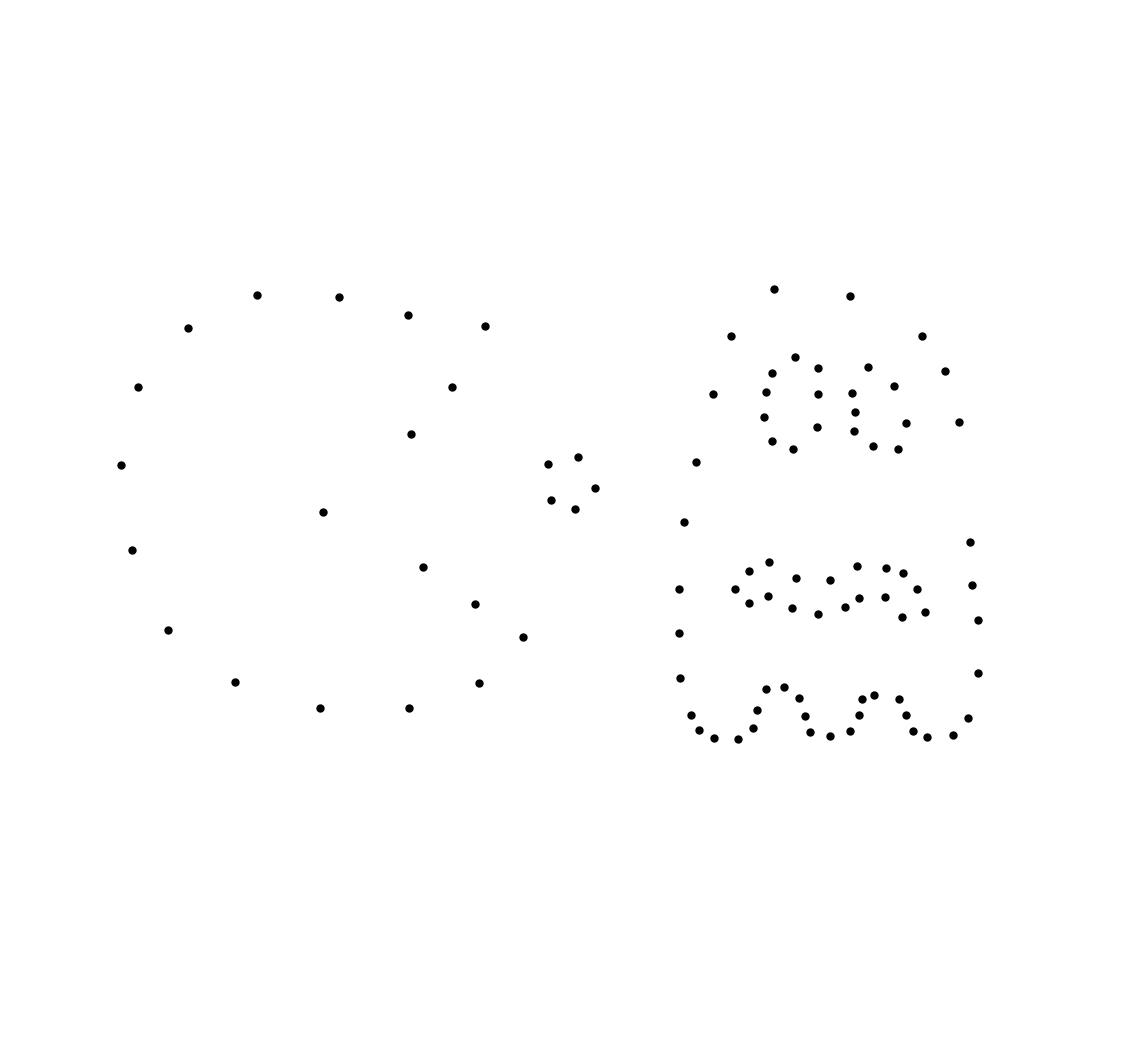
\includegraphics[width=\linewidth]{figure_source/crust_example_1a.png}
		\end{subfigure}
	}
	\hspace{0.2cm}
	\fbox{
		\begin{subfigure}{0.4\textwidth}
			\centering
			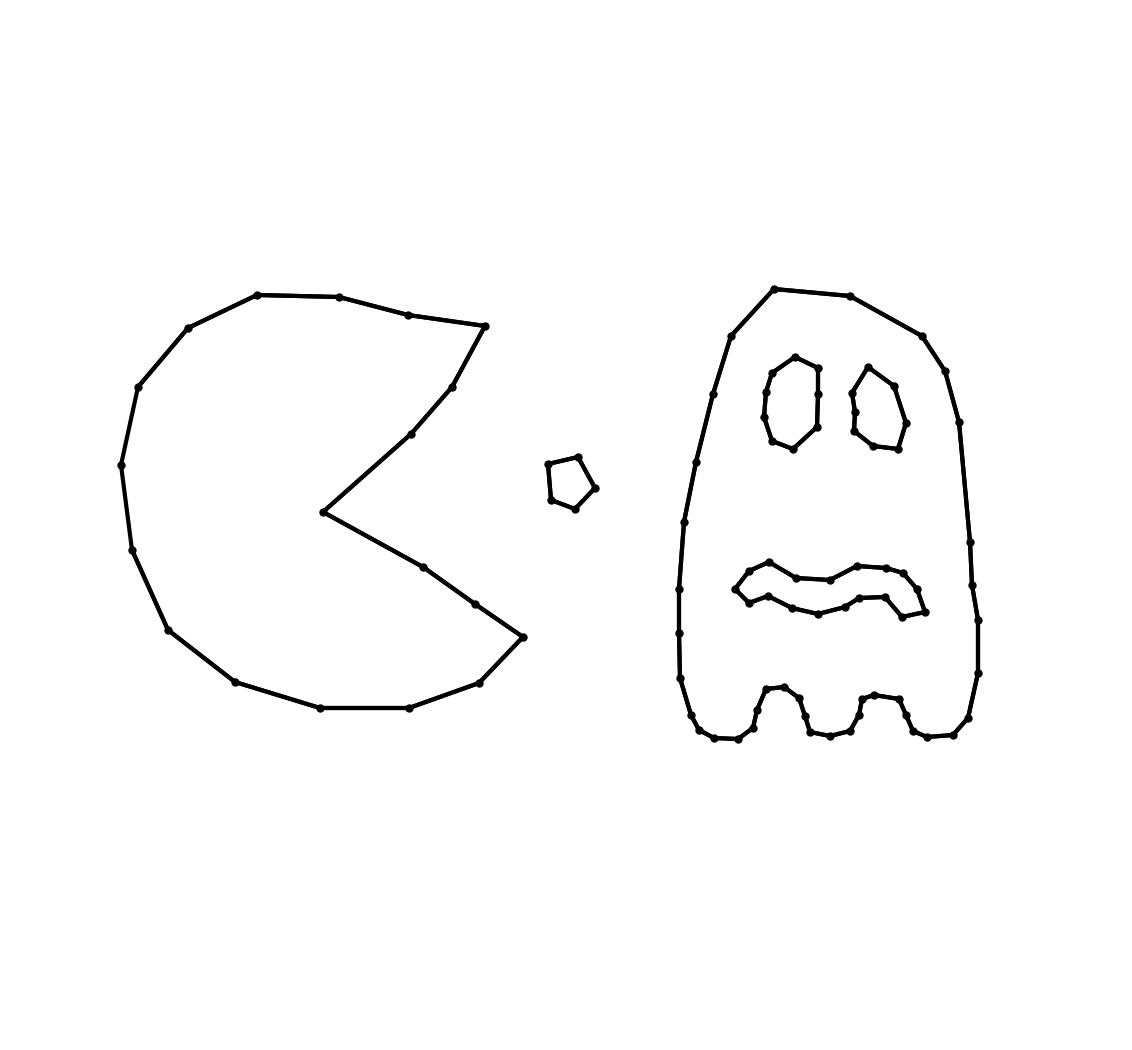
\includegraphics[width=\linewidth]{figure_source/crust_example_1b.png}
		\end{subfigure}
	}

	\caption{An example of the crust on a discrete set of points;}
	\label{fig:crust_example_1}
\end{figure}


To simplify the discussion in this paper, all sets of points in the plane are assumed to be in \textit{general position}.
General position can mean different things for different situations, but it essentially means points are not situated in a way that makes definitions ambiguous.
For example, it may be assumed that given a set of points $S$, you may split $S$ in half and take all those on the left and all those on the right.
In such a case, general position would mean that a line could be drawn that divides the points, rather than having multiple points in a vertical line in the middle.
Another example that is used repetitively in this paper is that no four points in $S$ can be connected by a circle.

